% Options for packages loaded elsewhere
% Options for packages loaded elsewhere
\PassOptionsToPackage{unicode}{hyperref}
\PassOptionsToPackage{hyphens}{url}
\PassOptionsToPackage{dvipsnames,svgnames,x11names}{xcolor}
%
\documentclass[
  letterpaper,
  DIV=11,
  numbers=noendperiod]{scrartcl}
\usepackage{xcolor}
\usepackage{amsmath,amssymb}
\setcounter{secnumdepth}{-\maxdimen} % remove section numbering
\usepackage{iftex}
\ifPDFTeX
  \usepackage[T1]{fontenc}
  \usepackage[utf8]{inputenc}
  \usepackage{textcomp} % provide euro and other symbols
\else % if luatex or xetex
  \usepackage{unicode-math} % this also loads fontspec
  \defaultfontfeatures{Scale=MatchLowercase}
  \defaultfontfeatures[\rmfamily]{Ligatures=TeX,Scale=1}
\fi
\usepackage{lmodern}
\ifPDFTeX\else
  % xetex/luatex font selection
\fi
% Use upquote if available, for straight quotes in verbatim environments
\IfFileExists{upquote.sty}{\usepackage{upquote}}{}
\IfFileExists{microtype.sty}{% use microtype if available
  \usepackage[]{microtype}
  \UseMicrotypeSet[protrusion]{basicmath} % disable protrusion for tt fonts
}{}
\makeatletter
\@ifundefined{KOMAClassName}{% if non-KOMA class
  \IfFileExists{parskip.sty}{%
    \usepackage{parskip}
  }{% else
    \setlength{\parindent}{0pt}
    \setlength{\parskip}{6pt plus 2pt minus 1pt}}
}{% if KOMA class
  \KOMAoptions{parskip=half}}
\makeatother
% Make \paragraph and \subparagraph free-standing
\makeatletter
\ifx\paragraph\undefined\else
  \let\oldparagraph\paragraph
  \renewcommand{\paragraph}{
    \@ifstar
      \xxxParagraphStar
      \xxxParagraphNoStar
  }
  \newcommand{\xxxParagraphStar}[1]{\oldparagraph*{#1}\mbox{}}
  \newcommand{\xxxParagraphNoStar}[1]{\oldparagraph{#1}\mbox{}}
\fi
\ifx\subparagraph\undefined\else
  \let\oldsubparagraph\subparagraph
  \renewcommand{\subparagraph}{
    \@ifstar
      \xxxSubParagraphStar
      \xxxSubParagraphNoStar
  }
  \newcommand{\xxxSubParagraphStar}[1]{\oldsubparagraph*{#1}\mbox{}}
  \newcommand{\xxxSubParagraphNoStar}[1]{\oldsubparagraph{#1}\mbox{}}
\fi
\makeatother

\usepackage{color}
\usepackage{fancyvrb}
\newcommand{\VerbBar}{|}
\newcommand{\VERB}{\Verb[commandchars=\\\{\}]}
\DefineVerbatimEnvironment{Highlighting}{Verbatim}{commandchars=\\\{\}}
% Add ',fontsize=\small' for more characters per line
\usepackage{framed}
\definecolor{shadecolor}{RGB}{241,243,245}
\newenvironment{Shaded}{\begin{snugshade}}{\end{snugshade}}
\newcommand{\AlertTok}[1]{\textcolor[rgb]{0.68,0.00,0.00}{#1}}
\newcommand{\AnnotationTok}[1]{\textcolor[rgb]{0.37,0.37,0.37}{#1}}
\newcommand{\AttributeTok}[1]{\textcolor[rgb]{0.40,0.45,0.13}{#1}}
\newcommand{\BaseNTok}[1]{\textcolor[rgb]{0.68,0.00,0.00}{#1}}
\newcommand{\BuiltInTok}[1]{\textcolor[rgb]{0.00,0.23,0.31}{#1}}
\newcommand{\CharTok}[1]{\textcolor[rgb]{0.13,0.47,0.30}{#1}}
\newcommand{\CommentTok}[1]{\textcolor[rgb]{0.37,0.37,0.37}{#1}}
\newcommand{\CommentVarTok}[1]{\textcolor[rgb]{0.37,0.37,0.37}{\textit{#1}}}
\newcommand{\ConstantTok}[1]{\textcolor[rgb]{0.56,0.35,0.01}{#1}}
\newcommand{\ControlFlowTok}[1]{\textcolor[rgb]{0.00,0.23,0.31}{\textbf{#1}}}
\newcommand{\DataTypeTok}[1]{\textcolor[rgb]{0.68,0.00,0.00}{#1}}
\newcommand{\DecValTok}[1]{\textcolor[rgb]{0.68,0.00,0.00}{#1}}
\newcommand{\DocumentationTok}[1]{\textcolor[rgb]{0.37,0.37,0.37}{\textit{#1}}}
\newcommand{\ErrorTok}[1]{\textcolor[rgb]{0.68,0.00,0.00}{#1}}
\newcommand{\ExtensionTok}[1]{\textcolor[rgb]{0.00,0.23,0.31}{#1}}
\newcommand{\FloatTok}[1]{\textcolor[rgb]{0.68,0.00,0.00}{#1}}
\newcommand{\FunctionTok}[1]{\textcolor[rgb]{0.28,0.35,0.67}{#1}}
\newcommand{\ImportTok}[1]{\textcolor[rgb]{0.00,0.46,0.62}{#1}}
\newcommand{\InformationTok}[1]{\textcolor[rgb]{0.37,0.37,0.37}{#1}}
\newcommand{\KeywordTok}[1]{\textcolor[rgb]{0.00,0.23,0.31}{\textbf{#1}}}
\newcommand{\NormalTok}[1]{\textcolor[rgb]{0.00,0.23,0.31}{#1}}
\newcommand{\OperatorTok}[1]{\textcolor[rgb]{0.37,0.37,0.37}{#1}}
\newcommand{\OtherTok}[1]{\textcolor[rgb]{0.00,0.23,0.31}{#1}}
\newcommand{\PreprocessorTok}[1]{\textcolor[rgb]{0.68,0.00,0.00}{#1}}
\newcommand{\RegionMarkerTok}[1]{\textcolor[rgb]{0.00,0.23,0.31}{#1}}
\newcommand{\SpecialCharTok}[1]{\textcolor[rgb]{0.37,0.37,0.37}{#1}}
\newcommand{\SpecialStringTok}[1]{\textcolor[rgb]{0.13,0.47,0.30}{#1}}
\newcommand{\StringTok}[1]{\textcolor[rgb]{0.13,0.47,0.30}{#1}}
\newcommand{\VariableTok}[1]{\textcolor[rgb]{0.07,0.07,0.07}{#1}}
\newcommand{\VerbatimStringTok}[1]{\textcolor[rgb]{0.13,0.47,0.30}{#1}}
\newcommand{\WarningTok}[1]{\textcolor[rgb]{0.37,0.37,0.37}{\textit{#1}}}

\usepackage{longtable,booktabs,array}
\usepackage{calc} % for calculating minipage widths
% Correct order of tables after \paragraph or \subparagraph
\usepackage{etoolbox}
\makeatletter
\patchcmd\longtable{\par}{\if@noskipsec\mbox{}\fi\par}{}{}
\makeatother
% Allow footnotes in longtable head/foot
\IfFileExists{footnotehyper.sty}{\usepackage{footnotehyper}}{\usepackage{footnote}}
\makesavenoteenv{longtable}
\usepackage{graphicx}
\makeatletter
\newsavebox\pandoc@box
\newcommand*\pandocbounded[1]{% scales image to fit in text height/width
  \sbox\pandoc@box{#1}%
  \Gscale@div\@tempa{\textheight}{\dimexpr\ht\pandoc@box+\dp\pandoc@box\relax}%
  \Gscale@div\@tempb{\linewidth}{\wd\pandoc@box}%
  \ifdim\@tempb\p@<\@tempa\p@\let\@tempa\@tempb\fi% select the smaller of both
  \ifdim\@tempa\p@<\p@\scalebox{\@tempa}{\usebox\pandoc@box}%
  \else\usebox{\pandoc@box}%
  \fi%
}
% Set default figure placement to htbp
\def\fps@figure{htbp}
\makeatother


% definitions for citeproc citations
\NewDocumentCommand\citeproctext{}{}
\NewDocumentCommand\citeproc{mm}{%
  \begingroup\def\citeproctext{#2}\cite{#1}\endgroup}
\makeatletter
 % allow citations to break across lines
 \let\@cite@ofmt\@firstofone
 % avoid brackets around text for \cite:
 \def\@biblabel#1{}
 \def\@cite#1#2{{#1\if@tempswa , #2\fi}}
\makeatother
\newlength{\cslhangindent}
\setlength{\cslhangindent}{1.5em}
\newlength{\csllabelwidth}
\setlength{\csllabelwidth}{3em}
\newenvironment{CSLReferences}[2] % #1 hanging-indent, #2 entry-spacing
 {\begin{list}{}{%
  \setlength{\itemindent}{0pt}
  \setlength{\leftmargin}{0pt}
  \setlength{\parsep}{0pt}
  % turn on hanging indent if param 1 is 1
  \ifodd #1
   \setlength{\leftmargin}{\cslhangindent}
   \setlength{\itemindent}{-1\cslhangindent}
  \fi
  % set entry spacing
  \setlength{\itemsep}{#2\baselineskip}}}
 {\end{list}}
\usepackage{calc}
\newcommand{\CSLBlock}[1]{\hfill\break\parbox[t]{\linewidth}{\strut\ignorespaces#1\strut}}
\newcommand{\CSLLeftMargin}[1]{\parbox[t]{\csllabelwidth}{\strut#1\strut}}
\newcommand{\CSLRightInline}[1]{\parbox[t]{\linewidth - \csllabelwidth}{\strut#1\strut}}
\newcommand{\CSLIndent}[1]{\hspace{\cslhangindent}#1}



\setlength{\emergencystretch}{3em} % prevent overfull lines

\providecommand{\tightlist}{%
  \setlength{\itemsep}{0pt}\setlength{\parskip}{0pt}}



 


\KOMAoption{captions}{tableheading}
\makeatletter
\@ifpackageloaded{tcolorbox}{}{\usepackage[skins,breakable]{tcolorbox}}
\@ifpackageloaded{fontawesome5}{}{\usepackage{fontawesome5}}
\definecolor{quarto-callout-color}{HTML}{909090}
\definecolor{quarto-callout-note-color}{HTML}{0758E5}
\definecolor{quarto-callout-important-color}{HTML}{CC1914}
\definecolor{quarto-callout-warning-color}{HTML}{EB9113}
\definecolor{quarto-callout-tip-color}{HTML}{00A047}
\definecolor{quarto-callout-caution-color}{HTML}{FC5300}
\definecolor{quarto-callout-color-frame}{HTML}{acacac}
\definecolor{quarto-callout-note-color-frame}{HTML}{4582ec}
\definecolor{quarto-callout-important-color-frame}{HTML}{d9534f}
\definecolor{quarto-callout-warning-color-frame}{HTML}{f0ad4e}
\definecolor{quarto-callout-tip-color-frame}{HTML}{02b875}
\definecolor{quarto-callout-caution-color-frame}{HTML}{fd7e14}
\makeatother
\makeatletter
\@ifpackageloaded{caption}{}{\usepackage{caption}}
\AtBeginDocument{%
\ifdefined\contentsname
  \renewcommand*\contentsname{Table of contents}
\else
  \newcommand\contentsname{Table of contents}
\fi
\ifdefined\listfigurename
  \renewcommand*\listfigurename{List of Figures}
\else
  \newcommand\listfigurename{List of Figures}
\fi
\ifdefined\listtablename
  \renewcommand*\listtablename{List of Tables}
\else
  \newcommand\listtablename{List of Tables}
\fi
\ifdefined\figurename
  \renewcommand*\figurename{Figure}
\else
  \newcommand\figurename{Figure}
\fi
\ifdefined\tablename
  \renewcommand*\tablename{Table}
\else
  \newcommand\tablename{Table}
\fi
}
\@ifpackageloaded{float}{}{\usepackage{float}}
\floatstyle{ruled}
\@ifundefined{c@chapter}{\newfloat{codelisting}{h}{lop}}{\newfloat{codelisting}{h}{lop}[chapter]}
\floatname{codelisting}{Listing}
\newcommand*\listoflistings{\listof{codelisting}{List of Listings}}
\makeatother
\makeatletter
\makeatother
\makeatletter
\@ifpackageloaded{caption}{}{\usepackage{caption}}
\@ifpackageloaded{subcaption}{}{\usepackage{subcaption}}
\makeatother
\usepackage{bookmark}
\IfFileExists{xurl.sty}{\usepackage{xurl}}{} % add URL line breaks if available
\urlstyle{same}
\hypersetup{
  pdftitle={Understanding a Simulated Tax Rate},
  colorlinks=true,
  linkcolor={blue},
  filecolor={Maroon},
  citecolor={Blue},
  urlcolor={Blue},
  pdfcreator={LaTeX via pandoc}}


\title{Understanding a Simulated Tax Rate}
\usepackage{etoolbox}
\makeatletter
\providecommand{\subtitle}[1]{% add subtitle to \maketitle
  \apptocmd{\@title}{\par {\large #1 \par}}{}{}
}
\makeatother
\subtitle{Project Lecture}
\author{}
\date{}
\begin{document}
\maketitle

% --- St Andrews brand colours for callout boxes ---
\definecolor{quarto-callout-note-color}{HTML}{007DC5}
\definecolor{quarto-callout-note-color-frame}{HTML}{007DC5}

\definecolor{quarto-callout-tip-color}{HTML}{00853F}
\definecolor{quarto-callout-tip-color-frame}{HTML}{00853F}

\definecolor{quarto-callout-caution-color}{HTML}{F5842B}
\definecolor{quarto-callout-caution-color-frame}{HTML}{F5842B}

\definecolor{quarto-callout-warning-color}{HTML}{EE312A}
\definecolor{quarto-callout-warning-color-frame}{HTML}{EE312A}

\definecolor{quarto-callout-important-color}{HTML}{7B439A}
\definecolor{quarto-callout-important-color-frame}{HTML}{7B439A}

% This approach is similar to: https://github.com/orgs/quarto-dev/discussions/13739; which added the following to the YAML section 
%  pdf:
%    include-before-body:
%      - text: |
%          \definecolor{quarto-callout-note-color}{HTML}{007DC5}
%          \definecolor{quarto-callout-tip-color}{HTML}{00853F}
%          \definecolor{quarto-callout-important-color}{HTML}{7B439A}
%          \definecolor{quarto-callout-caution-color}{HTML}{F5842B}
%          \definecolor{quarto-callout-warning-color}{HTML}{EE312A}
 
% But follows the advice of https://quarto.org/docs/output-formats/pdf-basics.html to add macros.tex section. 

% Alternatively, you follow this approach: https://enrico.spinielli.net/posts/2023-05-01-quarto-callout-hack/
% However, it edits the formatting of the PDF entirely instead of just adding a few changes. 
% If following this advice, you append the above to the end of the title.tex file. 



\subsection{Overview}\label{overview}

\begin{itemize}
\item
  Research question: what is the causal affect of an increase in taxes
  on:

  \begin{itemize}
  \tightlist
  \item
    charitable giving
  \item
    labour supply
  \item
    wealth
  \end{itemize}
\item
  Using data from the Consumer Expenditure survey (for US)

  \begin{itemize}
  \item
    years: 2016-2019 \(\Rightarrow\) \textbf{pooled cross section}.
  \item
    avoided 2020 due to Covid
  \end{itemize}
\end{itemize}

\subsection{Specification}\label{specification}

Linear regression model

\[
  y_{it} = \alpha + \beta tax_{it} + \mathbf{x}_{it}\gamma + u_{it}
\]

where,

\[
  tax_{it} = T(\mathbf{x}_{it},s,t)
\]

\textbf{Problem:}

\begin{itemize}
\item
  \(tax_{it}\) is endogeneous

  \begin{itemize}
  \tightlist
  \item
    determined by factors that are ``self-selected'':
    \(\mathbf{x}_{it}\), potentially \(s\)
  \end{itemize}
\item
  BUT \(tax_{it}\) is also determined by exogenous tax policy:
  \(T(\cdot,s,t)\)
\end{itemize}

\subsection{Simulated instrument}\label{simulated-instrument}

The literature on elasticity of taxable income (Gruber and Saez 2002)
asks a similar question:\footnote{The paper is available online:
  \href{https://www.sciencedirect.com/science/article/pii/S0047272701000858}{www.sciencedirect.com}}

\[
  y_{it} = \alpha + \tau tax_{it} + \mathbf{x}_{it}\eta + u_{it}
\]

Where \(y_{it}\) is reported taxable income and \(tax_{it}\) is the
net-of-tax rate (i.e.~1 minus tax rate)

\begin{itemize}
\tightlist
\item
  Important policy parameter for understanding how tax changes translate
  into changes in taxable income (i.e.~Laffer curve)
\end{itemize}

\subsection{Identification}\label{identification}

Since \(tax_{it}\) is endogenous

\begin{itemize}
\tightlist
\item
  Instrument:
\end{itemize}

\[
  sim_{it} = TAXSIM(\mathbf{x}_{it},s,t)
\]

\begin{itemize}
\item
  Predicted \(tax_{it}\) based on observable income \emph{in the
  previous period}
\item
  Paper use panel data from administrative tax records
\end{itemize}

\begin{tcolorbox}[enhanced jigsaw, colback=white, colframe=quarto-callout-warning-color-frame, breakable, toptitle=1mm, titlerule=0mm, coltitle=black, rightrule=.15mm, opacitybacktitle=0.6, left=2mm, leftrule=.75mm, title=\textcolor{quarto-callout-warning-color}{\faExclamationTriangle}\hspace{0.5em}{Warning}, bottomrule=.15mm, toprule=.15mm, colbacktitle=quarto-callout-warning-color!10!white, bottomtitle=1mm, opacityback=0, arc=.35mm]

This project takes inspiration from Gruber and Saez (2002), but we do
not have the same data structure. The authors use panel data to look at
changes in taxes at the individual/household level. There are other
useful examples of approaches to simulated instruments, like Grossman,
Tello-Trillo, and Willage (2022) from \href{tutorial-4.qmd}{Tutorial 4}.

\end{tcolorbox}

\subsection{Reduced form}\label{reduced-form}

For this exercise, you will not observe \(tax\).

\begin{itemize}
\item
  Can't conduct IV estimation
\item
  But, you can estimate the reduced form relationship
\end{itemize}

\[
  y_{it} = \delta + \beta sim_{it} + x_{it}\gamma + v_{it}
\]

\subsection{Identifying variation}\label{identifying-variation}

Suppose you regress \(y\) on \(sim\) alone

\[
  \beta^s = \frac{Cov(y_{it},sim_{it})}{Var(sim_{it})}
\]

What is the source of variation in \(sim_{it}\)?

\begin{enumerate}
\def\labelenumi{\arabic{enumi}.}
\item
  Endogenous factors
\item
  Exogenous factors
\end{enumerate}

\subsection{}\label{section}

If instead, you regress \(y\) on \(sim\) and a set of controls
\(\mathbf{x}\)

\[
  y_{it} = \delta + \beta sim_{it} + \mathbf{x}_{it}\gamma + v_{it}
\]

Then,

\[
    \beta = \frac{Cov(\tilde y_{it},\widetilde{sim}_{it})}{Var(\widetilde{sim}_{it})}
\]

where \(\widetilde{sim}_{it}\) is residual from regressing \(sim\) on
\(\mathbf{x}\)

\subsection{Controls}\label{controls}

So, the controls you choose are important!

\begin{itemize}
\tightlist
\item
  To ``isolate'' the exogenous variation in \(sim\) you need to control
  for the right factors.
\end{itemize}

\begin{tcolorbox}[enhanced jigsaw, colback=white, colframe=quarto-callout-caution-color-frame, breakable, toptitle=1mm, titlerule=0mm, coltitle=black, rightrule=.15mm, opacitybacktitle=0.6, left=2mm, leftrule=.75mm, title=\textcolor{quarto-callout-caution-color}{\faFire}\hspace{0.5em}{Income}, bottomrule=.15mm, toprule=.15mm, colbacktitle=quarto-callout-caution-color!10!white, bottomtitle=1mm, opacityback=0, arc=.35mm]

The primary determinant of taxes is income. In Gruber and Saez (2002)
the authors use panel data to control for income in the previous period.
Meaning income cannot be an outcome of the contemporaneous tax change.

In the paper, the simulated taxes for the current period are based on
current tax policy, but previous period's income.

\end{tcolorbox}

\subsection{Matching}\label{matching}

If you think about it from a matching perspective, the instrument plugs
a set of characteristics into a TAXSIM function\footnote{This is the
  name of the tax simulated used to construct the variable in the CEX.}

\[
  sim_{it} = TAXSIM(\mathbf{x}_{it},s,t)
\]

That takes as inputs:

\begin{itemize}
\item
  The household's characteristics
\item
  Their state
\item
  The year
\end{itemize}

\subsection{}\label{section-1}

If two households (\(i,i'\)) have the same \(\mathbf{x}\), live in the
same \(s\) state, in the same period \(t\),

\[
  TAXSIM(\mathbf{x}_{it},s,t) = TAXSIM(\mathbf{x}_{i't},s,t) 
\]

\textbf{Perfect match!}

If you hold \(\mathbf{x}\) fixed (e.g.~control for \(\mathbf{x}\)),

\begin{itemize}
\item
  with a single state and time period,
\item
  there is no (identifying) variation in \(sim\).
\end{itemize}

\subsection{Different jurisdictions}\label{different-jurisdictions}

But you could find two households (\(i,i'\)) with the same
\(\mathbf{x}\) in the same period \(t\) who live in different states
(\(s,s'\)):

\[
  TAXSIM(\mathbf{x}_{it},s,t) \neq TAXSIM(\mathbf{x}_{i't},s',t)
\]

\textbf{IF} the states have different tax policies.

\begin{itemize}
\item
  You now have variation in \(sim\) based on the state people live in.
\item
  With a single cross-section of data this would be the best you can do.
\item
  A concern might be that \emph{people choose where to live}.

  \begin{itemize}
  \item
    unobserved preferences that determine the outcome (giving, labour,
    wealth) may also determine decisions on where to live.
  \item
    e.g., people know that Florida has low taxes and is a nice place to
    retire
  \end{itemize}
\end{itemize}

\subsection{Repeated observations}\label{repeated-observations}

With repeated observations, you can do a bit better.

\begin{itemize}
\tightlist
\item
  You could find two households (\(i,i'\)) with the same \(\mathbf{x}\),
  \textbf{in the same state} \(s\), but different periods (\(t,t'\))
\end{itemize}

\[
  TAXSIM(\mathbf{x}_{it},s,t) \neq TAXSIM(\mathbf{x}_{i't'},s,t')
\] \textbf{IF} there is a \emph{policy change}.

\begin{itemize}
\item
  Ideally, you would like different states to enact different policy
  changes
\item
  At a minimum, you want the policy change to affect different groups of
  people differently.
\end{itemize}

\subsection{Policy change}\label{policy-change}

The reason you were provided with a pooled cross-section of data from
2016-2019 is the Tax Cuts and Jobs Act (effective 1 January 2018)

\pandocbounded{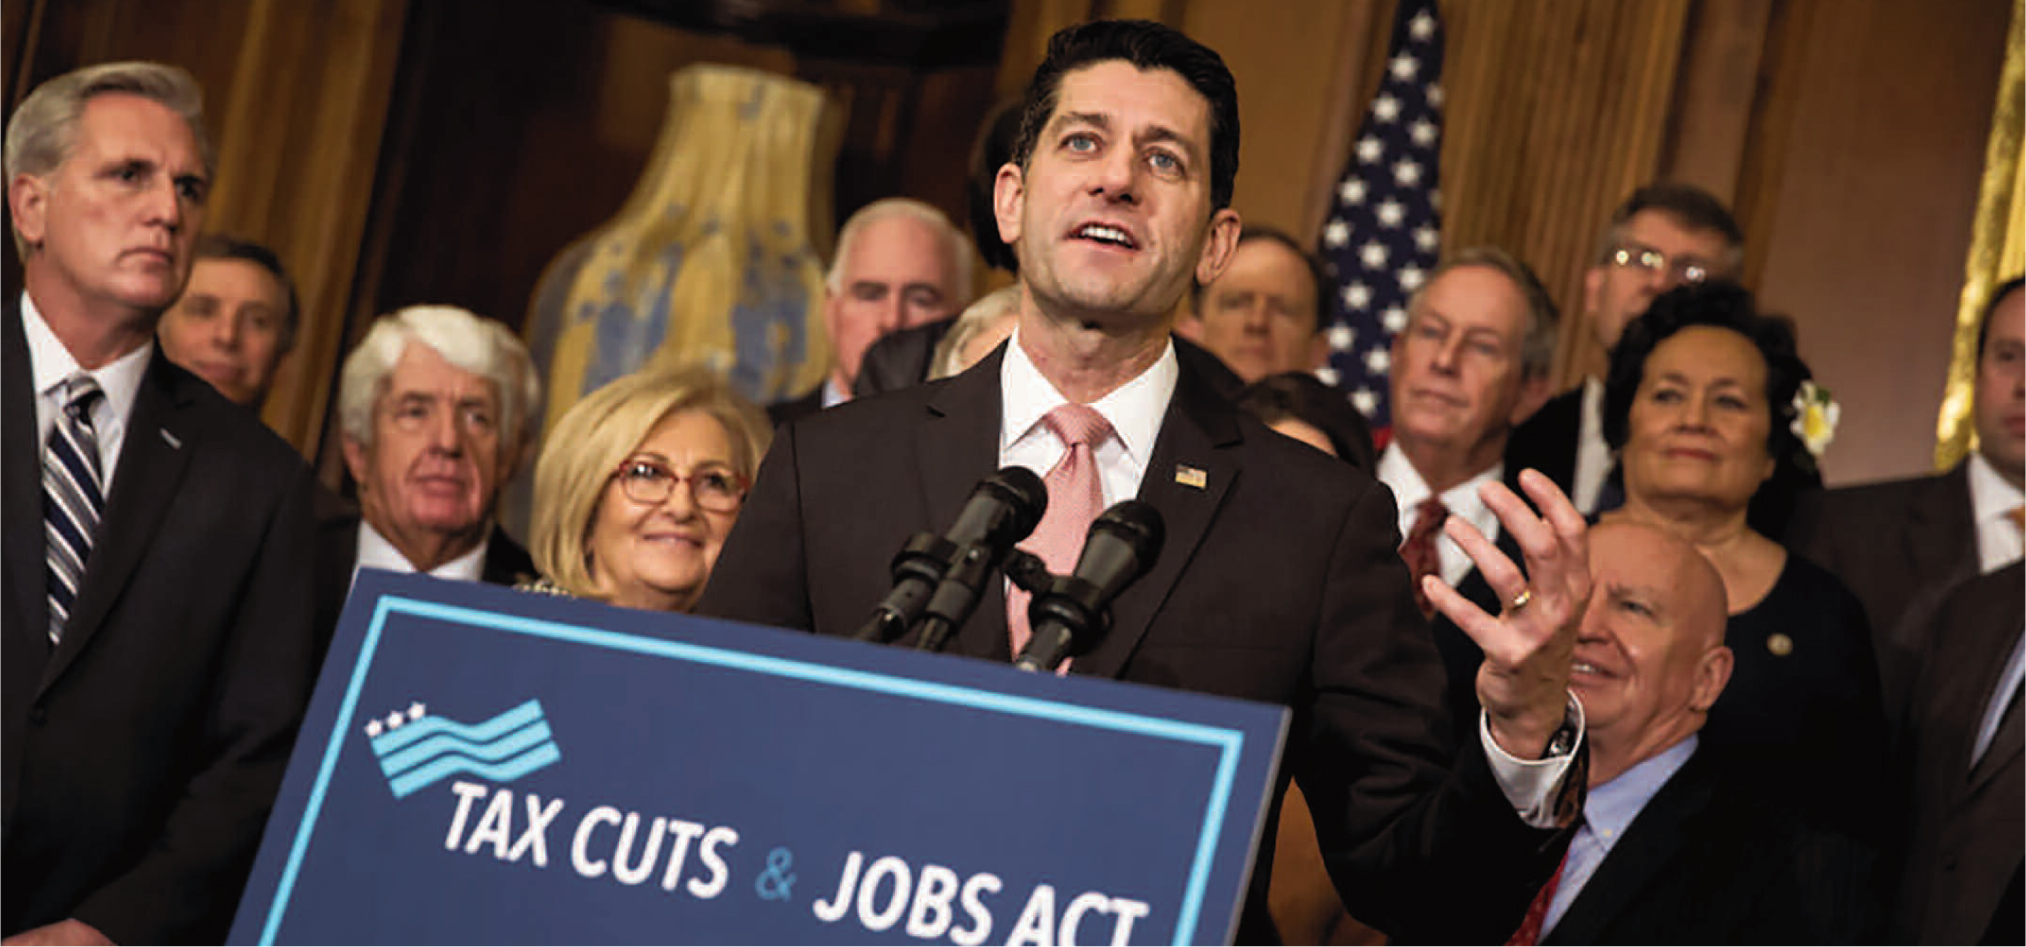
\includegraphics[keepaspectratio]{material/lecture-project/tax-cuts-jobs-act.jpg}}

\subsection{Simulation (1)}\label{simulation-1}

Simulation for single, 40-year-old, with USD 60,000 income

\begin{Shaded}
\begin{Highlighting}[]
\NormalTok{income }\OtherTok{\textless{}{-}} \DecValTok{60000}
\NormalTok{states }\OtherTok{\textless{}{-}} \FunctionTok{c}\NormalTok{(state.abb, }\StringTok{"DC"}\NormalTok{)   }\CommentTok{\# 50 states + DC}
\NormalTok{years  }\OtherTok{\textless{}{-}} \DecValTok{2016}\SpecialCharTok{:}\DecValTok{2019}

\CommentTok{\# {-}{-}{-}{-} 1. Build the TAXSIM input: one row per state{-}year {-}{-}{-}{-}{-}{-}{-}{-}{-}{-}{-}{-}{-}{-}{-}{-}{-}{-}{-}{-}{-}{-}}
\NormalTok{households }\OtherTok{\textless{}{-}} \FunctionTok{expand\_grid}\NormalTok{(}\AttributeTok{year =}\NormalTok{ years, }\AttributeTok{state =}\NormalTok{ states) }\SpecialCharTok{\%\textgreater{}\%}
  \FunctionTok{mutate}\NormalTok{(}\AttributeTok{taxsimid =} \FunctionTok{row\_number}\NormalTok{(),}
         \AttributeTok{mstat    =} \StringTok{"single"}\NormalTok{,}
         \AttributeTok{page     =} \DecValTok{40}\NormalTok{,       }\CommentTok{\# primary taxpayer\textquotesingle{}s age}
         \AttributeTok{depx     =} \DecValTok{0}\NormalTok{,        }\CommentTok{\# number of dependents}
         \AttributeTok{pwages   =}\NormalTok{ income)}

\CommentTok{\# {-}{-}{-}{-} 2. Calculate taxes {-}{-}{-}{-}{-}{-}{-}{-}{-}{-}{-}{-}{-}{-}{-}{-}{-}{-}{-}{-}{-}{-}{-}{-}{-}{-}{-}{-}{-}{-}{-}{-}{-}{-}{-}{-}{-}{-}{-}{-}{-}{-}{-}{-}{-}{-}{-}{-}{-}{-}{-}{-}{-}{-}}
\NormalTok{taxes }\OtherTok{\textless{}{-}} \FunctionTok{taxsim\_calculate\_taxes}\NormalTok{(households,}
                                \AttributeTok{marginal\_tax\_rates =} \StringTok{"Wages"}\NormalTok{)}

\CommentTok{\# {-}{-}{-}{-} 3. Average tax rates (\% of gross income) {-}{-}{-}{-}{-}{-}{-}{-}{-}{-}{-}{-}{-}{-}{-}{-}{-}{-}{-}{-}{-}{-}{-}{-}{-}{-}{-}{-}{-}{-}{-}{-}}
\NormalTok{rates }\OtherTok{\textless{}{-}}\NormalTok{ households }\SpecialCharTok{\%\textgreater{}\%}
  \FunctionTok{left\_join}\NormalTok{(taxes, }\AttributeTok{by =} \StringTok{"taxsimid"}\NormalTok{) }\SpecialCharTok{\%\textgreater{}\%}
  \FunctionTok{mutate}\NormalTok{(}\AttributeTok{federal\_atr =} \DecValTok{100} \SpecialCharTok{*}\NormalTok{ fiitax }\SpecialCharTok{/}\NormalTok{ pwages,}
         \AttributeTok{state\_atr   =} \DecValTok{100} \SpecialCharTok{*}\NormalTok{ siitax }\SpecialCharTok{/}\NormalTok{ pwages,}
         \AttributeTok{income\_atr  =}\NormalTok{ federal\_atr }\SpecialCharTok{+}\NormalTok{ state\_atr,}
         \AttributeTok{fica\_atr    =} \DecValTok{100} \SpecialCharTok{*}\NormalTok{ tfica }\SpecialCharTok{/}\NormalTok{ pwages,   }\CommentTok{\# employee share of payroll tax}
         \AttributeTok{total\_atr   =}\NormalTok{ income\_atr }\SpecialCharTok{+}\NormalTok{ fica\_atr)}

\CommentTok{\#write.csv(rates, "avg\_tax\_rate\_60k\_by\_state.csv", row.names = FALSE)}

\CommentTok{\# {-}{-}{-}{-} 4. Plot: one row per state, a dot per year {-}{-}{-}{-}{-}{-}{-}{-}{-}{-}{-}{-}{-}{-}{-}{-}{-}{-}{-}{-}{-}{-}{-}{-}{-}{-}{-}{-}{-}}
\CommentTok{\# Sort states by their 2019 rate}
\NormalTok{state\_order }\OtherTok{\textless{}{-}}\NormalTok{ rates }\SpecialCharTok{\%\textgreater{}\%}
  \FunctionTok{filter}\NormalTok{(year }\SpecialCharTok{==} \DecValTok{2019}\NormalTok{) }\SpecialCharTok{\%\textgreater{}\%}
  \FunctionTok{arrange}\NormalTok{(income\_atr) }\SpecialCharTok{\%\textgreater{}\%}
  \FunctionTok{pull}\NormalTok{(state)}

\NormalTok{plot\_data }\OtherTok{\textless{}{-}}\NormalTok{ rates }\SpecialCharTok{\%\textgreater{}\%}
  \FunctionTok{mutate}\NormalTok{(}\AttributeTok{state =} \FunctionTok{factor}\NormalTok{(state, }\AttributeTok{levels =}\NormalTok{ state\_order),}
         \AttributeTok{year  =} \FunctionTok{factor}\NormalTok{(year))}

\FunctionTok{ggplot}\NormalTok{(plot\_data, }\FunctionTok{aes}\NormalTok{(}\AttributeTok{x =}\NormalTok{ total\_atr, }\AttributeTok{y =}\NormalTok{ state)) }\SpecialCharTok{+}
  \FunctionTok{geom\_line}\NormalTok{(}\FunctionTok{aes}\NormalTok{(}\AttributeTok{group =}\NormalTok{ state), }\AttributeTok{colour =} \StringTok{"grey85"}\NormalTok{, }\AttributeTok{linewidth =} \FloatTok{0.8}\NormalTok{) }\SpecialCharTok{+}
  \FunctionTok{geom\_point}\NormalTok{(}\FunctionTok{aes}\NormalTok{(}\AttributeTok{colour =}\NormalTok{ year), }\AttributeTok{size =} \FloatTok{2.2}\NormalTok{) }\SpecialCharTok{+}
  \FunctionTok{scale\_colour\_manual}\NormalTok{(}\AttributeTok{values =} \FunctionTok{c}\NormalTok{(}\StringTok{"2016"} \OtherTok{=} \StringTok{"\#86b6ef"}\NormalTok{, }\StringTok{"2017"} \OtherTok{=} \StringTok{"\#3987e5"}\NormalTok{,}
                                 \StringTok{"2018"} \OtherTok{=} \StringTok{"\#1c5cab"}\NormalTok{, }\StringTok{"2019"} \OtherTok{=} \StringTok{"\#0d366b"}\NormalTok{)) }\SpecialCharTok{+}
  \FunctionTok{labs}\NormalTok{(}\AttributeTok{title    =} \StringTok{"Average income tax rate at $60,000 by state, 2016{-}2019"}\NormalTok{,}
       \AttributeTok{x        =} \StringTok{"Total income tax, \% of gross wages"}\NormalTok{,}
       \AttributeTok{y        =} \ConstantTok{NULL}\NormalTok{,}
       \AttributeTok{colour   =} \ConstantTok{NULL}\NormalTok{,}
       \AttributeTok{caption  =} \FunctionTok{paste}\NormalTok{(}\StringTok{"Single filer, age 40, no dependents, $60,000 wages."}\NormalTok{,}
                        \StringTok{"Includes local taxes and payroll tax."}\NormalTok{,}
                        \StringTok{"Source: NBER TAXSIM 35 via usincometaxes."}\NormalTok{,}
                        \AttributeTok{sep =} \StringTok{"}\SpecialCharTok{\textbackslash{}n}\StringTok{"}\NormalTok{)) }\SpecialCharTok{+}
  \FunctionTok{theme\_minimal}\NormalTok{(}\AttributeTok{base\_size =} \DecValTok{11}\NormalTok{) }\SpecialCharTok{+}
  \FunctionTok{theme}\NormalTok{(}\AttributeTok{legend.position     =} \StringTok{"top"}\NormalTok{,}
        \AttributeTok{panel.grid.major.y  =} \FunctionTok{element\_blank}\NormalTok{(),}
        \AttributeTok{panel.grid.minor    =} \FunctionTok{element\_blank}\NormalTok{(),}
        \AttributeTok{plot.caption        =} \FunctionTok{element\_text}\NormalTok{(}\AttributeTok{hjust =} \DecValTok{0}\NormalTok{, }\AttributeTok{colour =} \StringTok{"grey40"}\NormalTok{)) }\SpecialCharTok{+}
  \FunctionTok{scale\_x\_continuous}\NormalTok{(}\AttributeTok{limits =} \FunctionTok{c}\NormalTok{(}\DecValTok{0}\NormalTok{, }\DecValTok{50}\NormalTok{),}
                     \AttributeTok{breaks =} \FunctionTok{seq}\NormalTok{(}\DecValTok{0}\NormalTok{, }\DecValTok{50}\NormalTok{, }\AttributeTok{by =} \DecValTok{10}\NormalTok{),}
                     \AttributeTok{labels =} \ControlFlowTok{function}\NormalTok{(x) }\FunctionTok{paste0}\NormalTok{(x, }\StringTok{"\%"}\NormalTok{)) }\SpecialCharTok{+}
  \FunctionTok{scale\_y\_discrete}\NormalTok{(}\AttributeTok{guide =} \FunctionTok{guide\_axis}\NormalTok{(}\AttributeTok{n.dodge =} \DecValTok{2}\NormalTok{))}
\end{Highlighting}
\end{Shaded}

\pandocbounded{\includegraphics[keepaspectratio]{lecture-project_files/figure-pdf/unnamed-chunk-4-1.pdf}}

\subsection{Simulation (1)}\label{simulation-1-1}

Simulation for single, 40-year-old, with USD 120,000 income

\begin{Shaded}
\begin{Highlighting}[]
\CommentTok{\# {-}{-}{-}{-} 1. Build the TAXSIM input: one row per state{-}year {-}{-}{-}{-}{-}{-}{-}{-}{-}{-}{-}{-}{-}{-}{-}{-}{-}{-}{-}{-}{-}{-}}
\NormalTok{households }\OtherTok{\textless{}{-}} \FunctionTok{expand\_grid}\NormalTok{(}\AttributeTok{year =}\NormalTok{ years, }\AttributeTok{state =}\NormalTok{ states) }\SpecialCharTok{\%\textgreater{}\%}
  \FunctionTok{mutate}\NormalTok{(}\AttributeTok{taxsimid =} \FunctionTok{row\_number}\NormalTok{(),}
         \AttributeTok{mstat    =} \StringTok{"single"}\NormalTok{,}
         \AttributeTok{page     =} \DecValTok{40}\NormalTok{,       }\CommentTok{\# primary taxpayer\textquotesingle{}s age}
         \AttributeTok{depx     =} \DecValTok{0}\NormalTok{,        }\CommentTok{\# number of dependents}
         \AttributeTok{pwages   =}\NormalTok{ income}\SpecialCharTok{*}\DecValTok{2}\NormalTok{)}

\CommentTok{\# {-}{-}{-}{-} 2. Calculate taxes {-}{-}{-}{-}{-}{-}{-}{-}{-}{-}{-}{-}{-}{-}{-}{-}{-}{-}{-}{-}{-}{-}{-}{-}{-}{-}{-}{-}{-}{-}{-}{-}{-}{-}{-}{-}{-}{-}{-}{-}{-}{-}{-}{-}{-}{-}{-}{-}{-}{-}{-}{-}{-}{-}}
\NormalTok{taxes }\OtherTok{\textless{}{-}} \FunctionTok{taxsim\_calculate\_taxes}\NormalTok{(households,}
                                \AttributeTok{marginal\_tax\_rates =} \StringTok{"Wages"}\NormalTok{)}

\CommentTok{\# {-}{-}{-}{-} 3. Average tax rates (\% of gross income) {-}{-}{-}{-}{-}{-}{-}{-}{-}{-}{-}{-}{-}{-}{-}{-}{-}{-}{-}{-}{-}{-}{-}{-}{-}{-}{-}{-}{-}{-}{-}{-}}
\NormalTok{rates }\OtherTok{\textless{}{-}}\NormalTok{ households }\SpecialCharTok{\%\textgreater{}\%}
  \FunctionTok{left\_join}\NormalTok{(taxes, }\AttributeTok{by =} \StringTok{"taxsimid"}\NormalTok{) }\SpecialCharTok{\%\textgreater{}\%}
  \FunctionTok{mutate}\NormalTok{(}\AttributeTok{federal\_atr =} \DecValTok{100} \SpecialCharTok{*}\NormalTok{ fiitax }\SpecialCharTok{/}\NormalTok{ pwages,}
         \AttributeTok{state\_atr   =} \DecValTok{100} \SpecialCharTok{*}\NormalTok{ siitax }\SpecialCharTok{/}\NormalTok{ pwages,}
         \AttributeTok{income\_atr  =}\NormalTok{ federal\_atr }\SpecialCharTok{+}\NormalTok{ state\_atr,}
         \AttributeTok{fica\_atr    =} \DecValTok{100} \SpecialCharTok{*}\NormalTok{ tfica }\SpecialCharTok{/}\NormalTok{ pwages,   }\CommentTok{\# employee share of payroll tax}
         \AttributeTok{total\_atr   =}\NormalTok{ income\_atr }\SpecialCharTok{+}\NormalTok{ fica\_atr)}

\CommentTok{\#write.csv(rates, "avg\_tax\_rate\_60k\_by\_state.csv", row.names = FALSE)}

\CommentTok{\# {-}{-}{-}{-} 4. Plot: one row per state, a dot per year {-}{-}{-}{-}{-}{-}{-}{-}{-}{-}{-}{-}{-}{-}{-}{-}{-}{-}{-}{-}{-}{-}{-}{-}{-}{-}{-}{-}{-}}
\CommentTok{\# Sort states by their 2019 rate}
\NormalTok{state\_order }\OtherTok{\textless{}{-}}\NormalTok{ rates }\SpecialCharTok{\%\textgreater{}\%}
  \FunctionTok{filter}\NormalTok{(year }\SpecialCharTok{==} \DecValTok{2019}\NormalTok{) }\SpecialCharTok{\%\textgreater{}\%}
  \FunctionTok{arrange}\NormalTok{(income\_atr) }\SpecialCharTok{\%\textgreater{}\%}
  \FunctionTok{pull}\NormalTok{(state)}

\NormalTok{plot\_data }\OtherTok{\textless{}{-}}\NormalTok{ rates }\SpecialCharTok{\%\textgreater{}\%}
  \FunctionTok{mutate}\NormalTok{(}\AttributeTok{state =} \FunctionTok{factor}\NormalTok{(state, }\AttributeTok{levels =}\NormalTok{ state\_order),}
         \AttributeTok{year  =} \FunctionTok{factor}\NormalTok{(year))}

\FunctionTok{ggplot}\NormalTok{(plot\_data, }\FunctionTok{aes}\NormalTok{(}\AttributeTok{x =}\NormalTok{ total\_atr, }\AttributeTok{y =}\NormalTok{ state)) }\SpecialCharTok{+}
  \FunctionTok{geom\_line}\NormalTok{(}\FunctionTok{aes}\NormalTok{(}\AttributeTok{group =}\NormalTok{ state), }\AttributeTok{colour =} \StringTok{"grey85"}\NormalTok{, }\AttributeTok{linewidth =} \FloatTok{0.8}\NormalTok{) }\SpecialCharTok{+}
  \FunctionTok{geom\_point}\NormalTok{(}\FunctionTok{aes}\NormalTok{(}\AttributeTok{colour =}\NormalTok{ year), }\AttributeTok{size =} \FloatTok{2.2}\NormalTok{) }\SpecialCharTok{+}
  \FunctionTok{scale\_colour\_manual}\NormalTok{(}\AttributeTok{values =} \FunctionTok{c}\NormalTok{(}\StringTok{"2016"} \OtherTok{=} \StringTok{"\#86b6ef"}\NormalTok{, }\StringTok{"2017"} \OtherTok{=} \StringTok{"\#3987e5"}\NormalTok{,}
                                 \StringTok{"2018"} \OtherTok{=} \StringTok{"\#1c5cab"}\NormalTok{, }\StringTok{"2019"} \OtherTok{=} \StringTok{"\#0d366b"}\NormalTok{)) }\SpecialCharTok{+}
  \FunctionTok{labs}\NormalTok{(}\AttributeTok{title    =} \StringTok{"Average income tax rate at $120,000 by state, 2016{-}2019"}\NormalTok{,}
       \AttributeTok{x        =} \StringTok{"Total income tax, \% of gross wages"}\NormalTok{,}
       \AttributeTok{y        =} \ConstantTok{NULL}\NormalTok{,}
       \AttributeTok{colour   =} \ConstantTok{NULL}\NormalTok{,}
       \AttributeTok{caption  =} \FunctionTok{paste}\NormalTok{(}\StringTok{"Single filer, age 40, no dependents, $120,000 wages."}\NormalTok{,}
                        \StringTok{"Includes local taxes and payroll tax."}\NormalTok{,}
                        \StringTok{"Source: NBER TAXSIM 35 via usincometaxes."}\NormalTok{,}
                        \AttributeTok{sep =} \StringTok{"}\SpecialCharTok{\textbackslash{}n}\StringTok{"}\NormalTok{)) }\SpecialCharTok{+}
  \FunctionTok{theme\_minimal}\NormalTok{(}\AttributeTok{base\_size =} \DecValTok{11}\NormalTok{) }\SpecialCharTok{+}
  \FunctionTok{theme}\NormalTok{(}\AttributeTok{legend.position     =} \StringTok{"top"}\NormalTok{,}
        \AttributeTok{panel.grid.major.y  =} \FunctionTok{element\_blank}\NormalTok{(),}
        \AttributeTok{panel.grid.minor    =} \FunctionTok{element\_blank}\NormalTok{(),}
        \AttributeTok{plot.caption        =} \FunctionTok{element\_text}\NormalTok{(}\AttributeTok{hjust =} \DecValTok{0}\NormalTok{, }\AttributeTok{colour =} \StringTok{"grey40"}\NormalTok{)) }\SpecialCharTok{+}
  \FunctionTok{scale\_x\_continuous}\NormalTok{(}\AttributeTok{limits =} \FunctionTok{c}\NormalTok{(}\DecValTok{0}\NormalTok{, }\DecValTok{50}\NormalTok{),}
                     \AttributeTok{breaks =} \FunctionTok{seq}\NormalTok{(}\DecValTok{0}\NormalTok{, }\DecValTok{50}\NormalTok{, }\AttributeTok{by =} \DecValTok{10}\NormalTok{),}
                     \AttributeTok{labels =} \ControlFlowTok{function}\NormalTok{(x) }\FunctionTok{paste0}\NormalTok{(x, }\StringTok{"\%"}\NormalTok{)) }\SpecialCharTok{+}
  \FunctionTok{scale\_y\_discrete}\NormalTok{(}\AttributeTok{guide =} \FunctionTok{guide\_axis}\NormalTok{(}\AttributeTok{n.dodge =} \DecValTok{2}\NormalTok{))}
\end{Highlighting}
\end{Shaded}

\pandocbounded{\includegraphics[keepaspectratio]{lecture-project_files/figure-pdf/unnamed-chunk-5-1.pdf}}

\subsection{Simulation (3)}\label{simulation-3}

Simulation for married, 40-year-old couple, single-earner, 2 children
(ages 6 and 8), with USD 60,000 income

\begin{Shaded}
\begin{Highlighting}[]
\CommentTok{\# {-}{-}{-}{-} 1. Build the TAXSIM input: one row per state{-}year {-}{-}{-}{-}{-}{-}{-}{-}{-}{-}{-}{-}{-}{-}{-}{-}{-}{-}{-}{-}{-}{-}}
\NormalTok{households }\OtherTok{\textless{}{-}} \FunctionTok{expand\_grid}\NormalTok{(}\AttributeTok{year =}\NormalTok{ years, }\AttributeTok{state =}\NormalTok{ states) }\SpecialCharTok{\%\textgreater{}\%}
  \FunctionTok{mutate}\NormalTok{(}\AttributeTok{taxsimid =} \FunctionTok{row\_number}\NormalTok{(),}
         \AttributeTok{mstat    =} \StringTok{"married, jointly"}\NormalTok{,}
         \AttributeTok{page     =} \DecValTok{40}\NormalTok{,       }\CommentTok{\# primary taxpayer\textquotesingle{}s age}
         \AttributeTok{sage     =} \DecValTok{40}\NormalTok{,       }\CommentTok{\# spouse\textquotesingle{}s age}
         \AttributeTok{depx     =} \DecValTok{2}\NormalTok{,        }\CommentTok{\# number of dependents}
         \AttributeTok{age1     =} \DecValTok{6}\NormalTok{,       }\CommentTok{\# ages of the dependents}
         \AttributeTok{age2     =} \DecValTok{8}\NormalTok{,}
         \AttributeTok{pwages   =}\NormalTok{ income,   }\CommentTok{\# all wages earned by one spouse}
         \AttributeTok{swages   =} \DecValTok{0}\NormalTok{)}

\CommentTok{\# {-}{-}{-}{-} 2. Calculate taxes {-}{-}{-}{-}{-}{-}{-}{-}{-}{-}{-}{-}{-}{-}{-}{-}{-}{-}{-}{-}{-}{-}{-}{-}{-}{-}{-}{-}{-}{-}{-}{-}{-}{-}{-}{-}{-}{-}{-}{-}{-}{-}{-}{-}{-}{-}{-}{-}{-}{-}{-}{-}{-}{-}}
\NormalTok{taxes }\OtherTok{\textless{}{-}} \FunctionTok{taxsim\_calculate\_taxes}\NormalTok{(households,}
                                \AttributeTok{marginal\_tax\_rates =} \StringTok{"Wages"}\NormalTok{)}

\CommentTok{\# {-}{-}{-}{-} 3. Average tax rates (\% of gross income) {-}{-}{-}{-}{-}{-}{-}{-}{-}{-}{-}{-}{-}{-}{-}{-}{-}{-}{-}{-}{-}{-}{-}{-}{-}{-}{-}{-}{-}{-}{-}{-}}
\NormalTok{rates }\OtherTok{\textless{}{-}}\NormalTok{ households }\SpecialCharTok{\%\textgreater{}\%}
  \FunctionTok{left\_join}\NormalTok{(taxes, }\AttributeTok{by =} \StringTok{"taxsimid"}\NormalTok{) }\SpecialCharTok{\%\textgreater{}\%}
  \FunctionTok{mutate}\NormalTok{(}\AttributeTok{federal\_atr =} \DecValTok{100} \SpecialCharTok{*}\NormalTok{ fiitax }\SpecialCharTok{/}\NormalTok{ pwages,}
         \AttributeTok{state\_atr   =} \DecValTok{100} \SpecialCharTok{*}\NormalTok{ siitax }\SpecialCharTok{/}\NormalTok{ pwages,}
         \AttributeTok{income\_atr  =}\NormalTok{ federal\_atr }\SpecialCharTok{+}\NormalTok{ state\_atr,}
         \AttributeTok{fica\_atr    =} \DecValTok{100} \SpecialCharTok{*}\NormalTok{ tfica }\SpecialCharTok{/}\NormalTok{ pwages,   }\CommentTok{\# employee share of payroll tax}
         \AttributeTok{total\_atr   =}\NormalTok{ income\_atr }\SpecialCharTok{+}\NormalTok{ fica\_atr)}

\CommentTok{\#write.csv(rates, "avg\_tax\_rate\_60k\_by\_state.csv", row.names = FALSE)}

\CommentTok{\# {-}{-}{-}{-} 4. Plot: one row per state, a dot per year {-}{-}{-}{-}{-}{-}{-}{-}{-}{-}{-}{-}{-}{-}{-}{-}{-}{-}{-}{-}{-}{-}{-}{-}{-}{-}{-}{-}{-}}
\CommentTok{\# Sort states by their 2019 rate}
\NormalTok{state\_order }\OtherTok{\textless{}{-}}\NormalTok{ rates }\SpecialCharTok{\%\textgreater{}\%}
  \FunctionTok{filter}\NormalTok{(year }\SpecialCharTok{==} \DecValTok{2019}\NormalTok{) }\SpecialCharTok{\%\textgreater{}\%}
  \FunctionTok{arrange}\NormalTok{(income\_atr) }\SpecialCharTok{\%\textgreater{}\%}
  \FunctionTok{pull}\NormalTok{(state)}

\NormalTok{plot\_data }\OtherTok{\textless{}{-}}\NormalTok{ rates }\SpecialCharTok{\%\textgreater{}\%}
  \FunctionTok{mutate}\NormalTok{(}\AttributeTok{state =} \FunctionTok{factor}\NormalTok{(state, }\AttributeTok{levels =}\NormalTok{ state\_order),}
         \AttributeTok{year  =} \FunctionTok{factor}\NormalTok{(year))}

\FunctionTok{ggplot}\NormalTok{(plot\_data, }\FunctionTok{aes}\NormalTok{(}\AttributeTok{x =}\NormalTok{ total\_atr, }\AttributeTok{y =}\NormalTok{ state)) }\SpecialCharTok{+}
  \FunctionTok{geom\_line}\NormalTok{(}\FunctionTok{aes}\NormalTok{(}\AttributeTok{group =}\NormalTok{ state), }\AttributeTok{colour =} \StringTok{"grey85"}\NormalTok{, }\AttributeTok{linewidth =} \FloatTok{0.8}\NormalTok{) }\SpecialCharTok{+}
  \FunctionTok{geom\_point}\NormalTok{(}\FunctionTok{aes}\NormalTok{(}\AttributeTok{colour =}\NormalTok{ year), }\AttributeTok{size =} \FloatTok{2.2}\NormalTok{) }\SpecialCharTok{+}
  \FunctionTok{scale\_colour\_manual}\NormalTok{(}\AttributeTok{values =} \FunctionTok{c}\NormalTok{(}\StringTok{"2016"} \OtherTok{=} \StringTok{"\#86b6ef"}\NormalTok{, }\StringTok{"2017"} \OtherTok{=} \StringTok{"\#3987e5"}\NormalTok{,}
                                 \StringTok{"2018"} \OtherTok{=} \StringTok{"\#1c5cab"}\NormalTok{, }\StringTok{"2019"} \OtherTok{=} \StringTok{"\#0d366b"}\NormalTok{)) }\SpecialCharTok{+}
  \FunctionTok{labs}\NormalTok{(}\AttributeTok{title    =} \StringTok{"Average income tax rate at $60,000 by state, 2016{-}2019"}\NormalTok{,}
       \AttributeTok{x        =} \StringTok{"Total income tax, \% of gross wages"}\NormalTok{,}
       \AttributeTok{y        =} \ConstantTok{NULL}\NormalTok{,}
       \AttributeTok{colour   =} \ConstantTok{NULL}\NormalTok{,}
       \AttributeTok{caption  =} \FunctionTok{paste}\NormalTok{(}\StringTok{"Married filer, age 40, 2 dependents, $60,000 wages single earner."}\NormalTok{,}
                        \StringTok{"Includes local taxes and payroll tax."}\NormalTok{,}
                        \StringTok{"Source: NBER TAXSIM 35 via usincometaxes."}\NormalTok{,}
                        \AttributeTok{sep =} \StringTok{"}\SpecialCharTok{\textbackslash{}n}\StringTok{"}\NormalTok{)) }\SpecialCharTok{+}
  \FunctionTok{theme\_minimal}\NormalTok{(}\AttributeTok{base\_size =} \DecValTok{11}\NormalTok{) }\SpecialCharTok{+}
  \FunctionTok{theme}\NormalTok{(}\AttributeTok{legend.position     =} \StringTok{"top"}\NormalTok{,}
        \AttributeTok{panel.grid.major.y  =} \FunctionTok{element\_blank}\NormalTok{(),}
        \AttributeTok{panel.grid.minor    =} \FunctionTok{element\_blank}\NormalTok{(),}
        \AttributeTok{plot.caption        =} \FunctionTok{element\_text}\NormalTok{(}\AttributeTok{hjust =} \DecValTok{0}\NormalTok{, }\AttributeTok{colour =} \StringTok{"grey40"}\NormalTok{)) }\SpecialCharTok{+}
  \FunctionTok{scale\_x\_continuous}\NormalTok{(}\AttributeTok{limits =} \FunctionTok{c}\NormalTok{(}\DecValTok{0}\NormalTok{, }\DecValTok{50}\NormalTok{),}
                     \AttributeTok{breaks =} \FunctionTok{seq}\NormalTok{(}\DecValTok{0}\NormalTok{, }\DecValTok{50}\NormalTok{, }\AttributeTok{by =} \DecValTok{10}\NormalTok{),}
                     \AttributeTok{labels =} \ControlFlowTok{function}\NormalTok{(x) }\FunctionTok{paste0}\NormalTok{(x, }\StringTok{"\%"}\NormalTok{)) }\SpecialCharTok{+}
  \FunctionTok{scale\_y\_discrete}\NormalTok{(}\AttributeTok{guide =} \FunctionTok{guide\_axis}\NormalTok{(}\AttributeTok{n.dodge =} \DecValTok{2}\NormalTok{))}
\end{Highlighting}
\end{Shaded}

\pandocbounded{\includegraphics[keepaspectratio]{lecture-project_files/figure-pdf/unnamed-chunk-6-1.pdf}}

\subsection{Simulation (4)}\label{simulation-4}

Simulation for married, 40-year-old couple, double-earner, 2 children
(ages 6 and 8), with USD 60,000 income \textbf{each}

\begin{Shaded}
\begin{Highlighting}[]
\CommentTok{\# {-}{-}{-}{-} 1. Build the TAXSIM input: one row per state{-}year {-}{-}{-}{-}{-}{-}{-}{-}{-}{-}{-}{-}{-}{-}{-}{-}{-}{-}{-}{-}{-}{-}}
\NormalTok{households }\OtherTok{\textless{}{-}} \FunctionTok{expand\_grid}\NormalTok{(}\AttributeTok{year =}\NormalTok{ years, }\AttributeTok{state =}\NormalTok{ states) }\SpecialCharTok{\%\textgreater{}\%}
  \FunctionTok{mutate}\NormalTok{(}\AttributeTok{taxsimid =} \FunctionTok{row\_number}\NormalTok{(),}
         \AttributeTok{mstat    =} \StringTok{"married, jointly"}\NormalTok{,}
         \AttributeTok{page     =} \DecValTok{40}\NormalTok{,       }\CommentTok{\# primary taxpayer\textquotesingle{}s age}
         \AttributeTok{sage     =} \DecValTok{40}\NormalTok{,       }\CommentTok{\# spouse\textquotesingle{}s age}
         \AttributeTok{depx     =} \DecValTok{2}\NormalTok{,        }\CommentTok{\# number of dependents}
         \AttributeTok{age1     =} \DecValTok{6}\NormalTok{,       }\CommentTok{\# ages of the dependents}
         \AttributeTok{age2     =} \DecValTok{8}\NormalTok{,}
         \AttributeTok{pwages   =}\NormalTok{ income,   }\CommentTok{\# all wages earned by one spouse}
         \AttributeTok{swages   =}\NormalTok{ income)}

\CommentTok{\# {-}{-}{-}{-} 2. Calculate taxes {-}{-}{-}{-}{-}{-}{-}{-}{-}{-}{-}{-}{-}{-}{-}{-}{-}{-}{-}{-}{-}{-}{-}{-}{-}{-}{-}{-}{-}{-}{-}{-}{-}{-}{-}{-}{-}{-}{-}{-}{-}{-}{-}{-}{-}{-}{-}{-}{-}{-}{-}{-}{-}{-}}
\NormalTok{taxes }\OtherTok{\textless{}{-}} \FunctionTok{taxsim\_calculate\_taxes}\NormalTok{(households,}
                                \AttributeTok{marginal\_tax\_rates =} \StringTok{"Wages"}\NormalTok{)}

\CommentTok{\# {-}{-}{-}{-} 3. Average tax rates (\% of gross income) {-}{-}{-}{-}{-}{-}{-}{-}{-}{-}{-}{-}{-}{-}{-}{-}{-}{-}{-}{-}{-}{-}{-}{-}{-}{-}{-}{-}{-}{-}{-}{-}}
\NormalTok{rates }\OtherTok{\textless{}{-}}\NormalTok{ households }\SpecialCharTok{\%\textgreater{}\%}
  \FunctionTok{left\_join}\NormalTok{(taxes, }\AttributeTok{by =} \StringTok{"taxsimid"}\NormalTok{) }\SpecialCharTok{\%\textgreater{}\%}
  \FunctionTok{mutate}\NormalTok{(}\AttributeTok{federal\_atr =} \DecValTok{100} \SpecialCharTok{*}\NormalTok{ fiitax }\SpecialCharTok{/}\NormalTok{ pwages,}
         \AttributeTok{state\_atr   =} \DecValTok{100} \SpecialCharTok{*}\NormalTok{ siitax }\SpecialCharTok{/}\NormalTok{ pwages,}
         \AttributeTok{income\_atr  =}\NormalTok{ federal\_atr }\SpecialCharTok{+}\NormalTok{ state\_atr,}
         \AttributeTok{fica\_atr    =} \DecValTok{100} \SpecialCharTok{*}\NormalTok{ tfica }\SpecialCharTok{/}\NormalTok{ pwages,   }\CommentTok{\# employee share of payroll tax}
         \AttributeTok{total\_atr   =}\NormalTok{ income\_atr }\SpecialCharTok{+}\NormalTok{ fica\_atr)}

\CommentTok{\#write.csv(rates, "avg\_tax\_rate\_60k\_by\_state.csv", row.names = FALSE)}

\CommentTok{\# {-}{-}{-}{-} 4. Plot: one row per state, a dot per year {-}{-}{-}{-}{-}{-}{-}{-}{-}{-}{-}{-}{-}{-}{-}{-}{-}{-}{-}{-}{-}{-}{-}{-}{-}{-}{-}{-}{-}}
\CommentTok{\# Sort states by their 2019 rate}
\NormalTok{state\_order }\OtherTok{\textless{}{-}}\NormalTok{ rates }\SpecialCharTok{\%\textgreater{}\%}
  \FunctionTok{filter}\NormalTok{(year }\SpecialCharTok{==} \DecValTok{2019}\NormalTok{) }\SpecialCharTok{\%\textgreater{}\%}
  \FunctionTok{arrange}\NormalTok{(income\_atr) }\SpecialCharTok{\%\textgreater{}\%}
  \FunctionTok{pull}\NormalTok{(state)}

\NormalTok{plot\_data }\OtherTok{\textless{}{-}}\NormalTok{ rates }\SpecialCharTok{\%\textgreater{}\%}
  \FunctionTok{mutate}\NormalTok{(}\AttributeTok{state =} \FunctionTok{factor}\NormalTok{(state, }\AttributeTok{levels =}\NormalTok{ state\_order),}
         \AttributeTok{year  =} \FunctionTok{factor}\NormalTok{(year))}

\FunctionTok{ggplot}\NormalTok{(plot\_data, }\FunctionTok{aes}\NormalTok{(}\AttributeTok{x =}\NormalTok{ total\_atr, }\AttributeTok{y =}\NormalTok{ state)) }\SpecialCharTok{+}
  \FunctionTok{geom\_line}\NormalTok{(}\FunctionTok{aes}\NormalTok{(}\AttributeTok{group =}\NormalTok{ state), }\AttributeTok{colour =} \StringTok{"grey85"}\NormalTok{, }\AttributeTok{linewidth =} \FloatTok{0.8}\NormalTok{) }\SpecialCharTok{+}
  \FunctionTok{geom\_point}\NormalTok{(}\FunctionTok{aes}\NormalTok{(}\AttributeTok{colour =}\NormalTok{ year), }\AttributeTok{size =} \FloatTok{2.2}\NormalTok{) }\SpecialCharTok{+}
  \FunctionTok{scale\_colour\_manual}\NormalTok{(}\AttributeTok{values =} \FunctionTok{c}\NormalTok{(}\StringTok{"2016"} \OtherTok{=} \StringTok{"\#86b6ef"}\NormalTok{, }\StringTok{"2017"} \OtherTok{=} \StringTok{"\#3987e5"}\NormalTok{,}
                                 \StringTok{"2018"} \OtherTok{=} \StringTok{"\#1c5cab"}\NormalTok{, }\StringTok{"2019"} \OtherTok{=} \StringTok{"\#0d366b"}\NormalTok{)) }\SpecialCharTok{+}
  \FunctionTok{labs}\NormalTok{(}\AttributeTok{title    =} \StringTok{"Average income tax rate at $120,000 by state, 2016{-}2019"}\NormalTok{,}
       \AttributeTok{x        =} \StringTok{"Total tax, \% of gross wages"}\NormalTok{,}
       \AttributeTok{y        =} \ConstantTok{NULL}\NormalTok{,}
       \AttributeTok{colour   =} \ConstantTok{NULL}\NormalTok{,}
       \AttributeTok{caption  =} \FunctionTok{paste}\NormalTok{(}\StringTok{"Married filer, age 40, 2 dependents, $60,000 wages both earners."}\NormalTok{,}
                        \StringTok{"Includes local taxes and payroll tax."}\NormalTok{,}
                        \StringTok{"Source: NBER TAXSIM 35 via usincometaxes."}\NormalTok{,}
                        \AttributeTok{sep =} \StringTok{"}\SpecialCharTok{\textbackslash{}n}\StringTok{"}\NormalTok{)) }\SpecialCharTok{+}
  \FunctionTok{theme\_minimal}\NormalTok{(}\AttributeTok{base\_size =} \DecValTok{11}\NormalTok{) }\SpecialCharTok{+}
  \FunctionTok{theme}\NormalTok{(}\AttributeTok{legend.position     =} \StringTok{"top"}\NormalTok{,}
        \AttributeTok{panel.grid.major.y  =} \FunctionTok{element\_blank}\NormalTok{(),}
        \AttributeTok{panel.grid.minor    =} \FunctionTok{element\_blank}\NormalTok{(),}
        \AttributeTok{plot.caption        =} \FunctionTok{element\_text}\NormalTok{(}\AttributeTok{hjust =} \DecValTok{0}\NormalTok{, }\AttributeTok{colour =} \StringTok{"grey40"}\NormalTok{)) }\SpecialCharTok{+}
  \FunctionTok{scale\_x\_continuous}\NormalTok{(}\AttributeTok{limits =} \FunctionTok{c}\NormalTok{(}\DecValTok{0}\NormalTok{, }\DecValTok{50}\NormalTok{),}
                     \AttributeTok{breaks =} \FunctionTok{seq}\NormalTok{(}\DecValTok{0}\NormalTok{, }\DecValTok{50}\NormalTok{, }\AttributeTok{by =} \DecValTok{10}\NormalTok{),}
                     \AttributeTok{labels =} \ControlFlowTok{function}\NormalTok{(x) }\FunctionTok{paste0}\NormalTok{(x, }\StringTok{"\%"}\NormalTok{)) }\SpecialCharTok{+}
  \FunctionTok{scale\_y\_discrete}\NormalTok{(}\AttributeTok{guide =} \FunctionTok{guide\_axis}\NormalTok{(}\AttributeTok{n.dodge =} \DecValTok{2}\NormalTok{))}
\end{Highlighting}
\end{Shaded}

\pandocbounded{\includegraphics[keepaspectratio]{lecture-project_files/figure-pdf/unnamed-chunk-7-1.pdf}}

\subsection{CEX (2016-2019)}\label{cex-2016-2019}

The data at your disposal is a repeated cross section of
\textbf{households}.

\begin{itemize}
\item
  In the CEX, households are surveyed four times (i.e.~a panel), but
  only the final interview asks about wealth. This is the one you
  observe.
\item
  Income is also recorded in the final interview.

  \begin{itemize}
  \item
    it represents the previous 12 months' income (i.e.~partly lagged, by
    up to 12 months)
  \item
    may not span an exact calendar/tax year.
  \end{itemize}
\item
  The tax variables are a weighted average of taxes for overlapping tax
  years,

  \begin{itemize}
  \item
    based on the months reported in each tax year
  \item
    \textbf{not ideal}, but does include some exogenous variation
    resulting from policy reforms
  \item
    you really see tax change taking effect in 2019 data, as 2018 income
    records partly reflect 2017 income.
  \end{itemize}
\end{itemize}

\subsection{CEX Plots}\label{cex-plots}

\begin{Shaded}
\begin{Highlighting}[]
\KeywordTok{use} \StringTok{"$data\_dir\textbackslash{}cex2016\_2019.dta"}\NormalTok{, }\KeywordTok{clear}

\KeywordTok{drop} \KeywordTok{if}\NormalTok{ state\_fips==.}
\KeywordTok{drop} \KeywordTok{if} \FunctionTok{inlist}\NormalTok{(state\_fips,54,33,18,19,10,11)}
\KeywordTok{drop} \KeywordTok{if}\NormalTok{ atr\_total\textless{}0 | atr\_total\textgreater{}1}

\KeywordTok{collapse}\NormalTok{ (}\KeywordTok{mean}\NormalTok{) atr\_total, }\KeywordTok{by}\NormalTok{(region release\_year)}

\NormalTok{xtset region release\_year}
\end{Highlighting}
\end{Shaded}

\begin{Shaded}
\begin{Highlighting}[]
\KeywordTok{xtline}\NormalTok{ atr\_total, overlay }\BaseNTok{xtitle}\NormalTok{(Survey Year) }\BaseNTok{ytitle}\NormalTok{(Average }\KeywordTok{of}\NormalTok{ atr\_total) }\KeywordTok{ylabel}\NormalTok{(0.05(0.05)0.15) }\BaseNTok{legend}\NormalTok{(pos(2) }\BaseNTok{ring}\NormalTok{(0)) }\BaseNTok{title}\NormalTok{(}\StringTok{"Selecting on households within incomes $30,000 to $120,000"}\NormalTok{)}
\end{Highlighting}
\end{Shaded}

\pandocbounded{\includegraphics[keepaspectratio]{lecture-project_files/mediabag/lecture-project_files/figure-pdf/unnamed-chunk-9-1.pdf}}

\subsection*{Bibliography}\label{bibliography}
\addcontentsline{toc}{subsection}{Bibliography}

\phantomsection\label{refs}
\begin{CSLReferences}{1}{0}
\bibitem[\citeproctext]{ref-grossman2022health}
Grossman, Daniel S, Sebastian Tello-Trillo, and Barton Willage. 2022.
{``Health Insurance for Whom? The `Spill-up'effects of Children's Health
Insurance on Mothers.''} National Bureau of Economic Research.

\bibitem[\citeproctext]{ref-gruber2002elasticity}
Gruber, Jon, and Emmanuel Saez. 2002. {``The Elasticity of Taxable
Income: Evidence and Implications.''} \emph{Journal of Public Economics}
84 (1): 1--32.

\end{CSLReferences}




\end{document}
